\section{Experiment}

\begin{figure}[t]
    \centering
    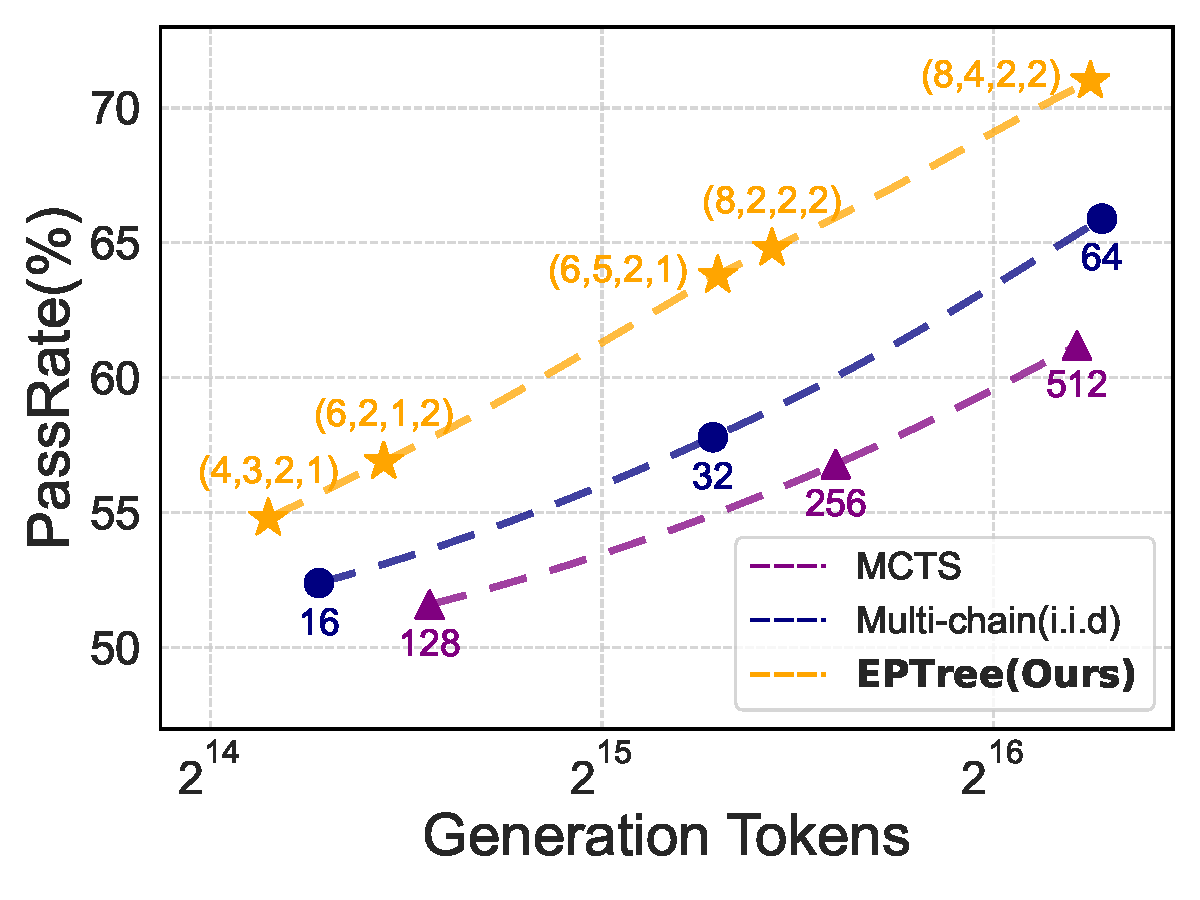
\includegraphics[width=0.45\textwidth]{figure/tree_iid_mcts_performance.pdf}
    \label{fig:tree_vs_iid_performance}
    \caption{Search performance of \treemodel, MCTS, and multi-chain sampling on Omni-MATH-500 using Qwen-2.5-14B-SFT. \treemodel consistently outperforms all baselines under the different inference costs. 
    % A detailed evaluation of \treemodel can be found in \Cref{sec:appendix:eptree_table}.
    }
    \vspace{-4mm}
    \label{fig:tree_vs_mcts_iid}
\end{figure}


\begin{table*}[!t]
    \caption{Experiment results on math reasoning tasks. We report Accuracy(\%) for all datasets.}
    \centering
    \resizebox{0.95\textwidth}{!}{%
        \begin{tabular}{lccccccc}
        \toprule[1.2pt]
             & MATH500 & \makecell{Omni-MA\\TH-500} & AIME2024 & AMC & \makecell{Olympiad\\Bench} & \makecell{LiveCode\\Bench} & Avg \\
         \midrule
         GPT-4o & 76.6 & 26.8 & 9.3 & 45.8 & 43.3 & 29.5 & 38.6 \\
         Llama-3.1-8B-Instruct & 52.8 & 15.0 & 10.9 & 22.6 & 15.6 & 11.6 & 21.4 \\
         Llama-3.3-70B-Instruct & 73.9 & 27.9 & 24.2 & 50.9 & 35.7 & 25.5 & 39.7 \\
         GLM4-9B-chat & 50.1 & 12.9 & 1.7 & 17.2 & 14.7 & 16.5 & 18.9 \\
         Qwen-2.5-7B-Instruct & 76.5 & 26.0 & 13.3 & 41.9 & 35.0 & 16.8 & 34.9 \\
         Qwen-2.5-Math-7B-Instruct & 82.7 & 29.7 & 16.7 & 50.6 & 40.7 & 8.1 & 38.1 \\
         Qwen-2.5-14B-Instruct & 78.9 & 28.7 & 13.7 & 54.5 & 41.8 & 27.7 & 40.9 \\
         % QwQ-32B-preview & 90.6 & 46.6 & 50.0 & 77.4 & 59.1 & 43.5 & 61.2 \\
         \midrule
         SFT (GLM-9B) & 56.0 & 18.2 & 8.3 & 29.2 & 22.5 & 14.2 & 24.7  \\
         ChainRL (GLM-9B)  & 63.0 & 21.8 & 6.1 & 31.6 & 23.9 & 16.6 & 27.2 \\
         \model (GLM-9B) & 64.5 & 20.8 & 11.4 & 38.5 & 24.8 & 15.8 & \textbf{29.3} \\
         \midrule
         SFT (Qwen-2.5-14B) & 76.6 & 29.5 & 10.6 & 48.0 & 36.9 & 14.5 & 36.0 \\
         ChainRL (Qwen-2.5-14B) & 81.6 & 32.7 & 22.2 & 53.9 & 41.1 & 18.2 & 41.6\\
         \model (Qwen-2.5-14B) & 81.7 & 36.7 & 28.0 & 55.9 & 44.6 & 20.8 & \textbf{44.5} \\
         \midrule
         SFT (R1-Distilled-Qwen-2.5-7B) & 94.0 & 47.8 & 55.9 & 85.5 & 54.4 & 43.9 & 63.6 \\
         ChainRL (R1-Distilled-Qwen-2.5-7B) & 93.6 & 48.1 & 59.7 & 85.5 & 54.5 & 46.1 & 64.5\\
         \model (R1-Distilled-Qwen-2.5-7B) & 94.4 & 49.8 & 60.8 & 85.0 & 57.1 & 47.4 & \textbf{65.8} \\
         \bottomrule[1.2pt]
        \end{tabular}
    }
    \label{tab:experiments}
\end{table*}




\begin{figure*}[!h]
    \centering
    \subfloat[Experiments on  Qwen-2.5-14B \label{subfig:a}]{
        \begin{minipage}{\textwidth}
            \centering
            \begin{minipage}{0.32\textwidth}
                \centering
                
\includegraphics[width=\textwidth]{figure/qwen-rlresult/average.pdf}
                \vspace{-5mm}
                \label{fig:first_image}
            \end{minipage}
            \hfill
            \begin{minipage}{0.32\textwidth}
                \centering
                
\includegraphics[width=\textwidth]{figure/qwen-rlresult/olympaidbench.pdf}
                \vspace{-5mm}
                \label{fig:second_image}
            \end{minipage}
            \hfill
            \begin{minipage}{0.32\textwidth}
                \centering
                
\includegraphics[width=\textwidth]{figure/qwen-rlresult/omni.pdf}
                \vspace{-5mm}
                \label{fig:third_image}
            \end{minipage}
        \end{minipage}
    }
    \vspace{1mm}
    \subfloat[Experiments on GLM4-9B \label{subfig:b}]{
        \begin{minipage}{\textwidth}
            \centering
            \begin{minipage}{0.32\textwidth}
                \centering
                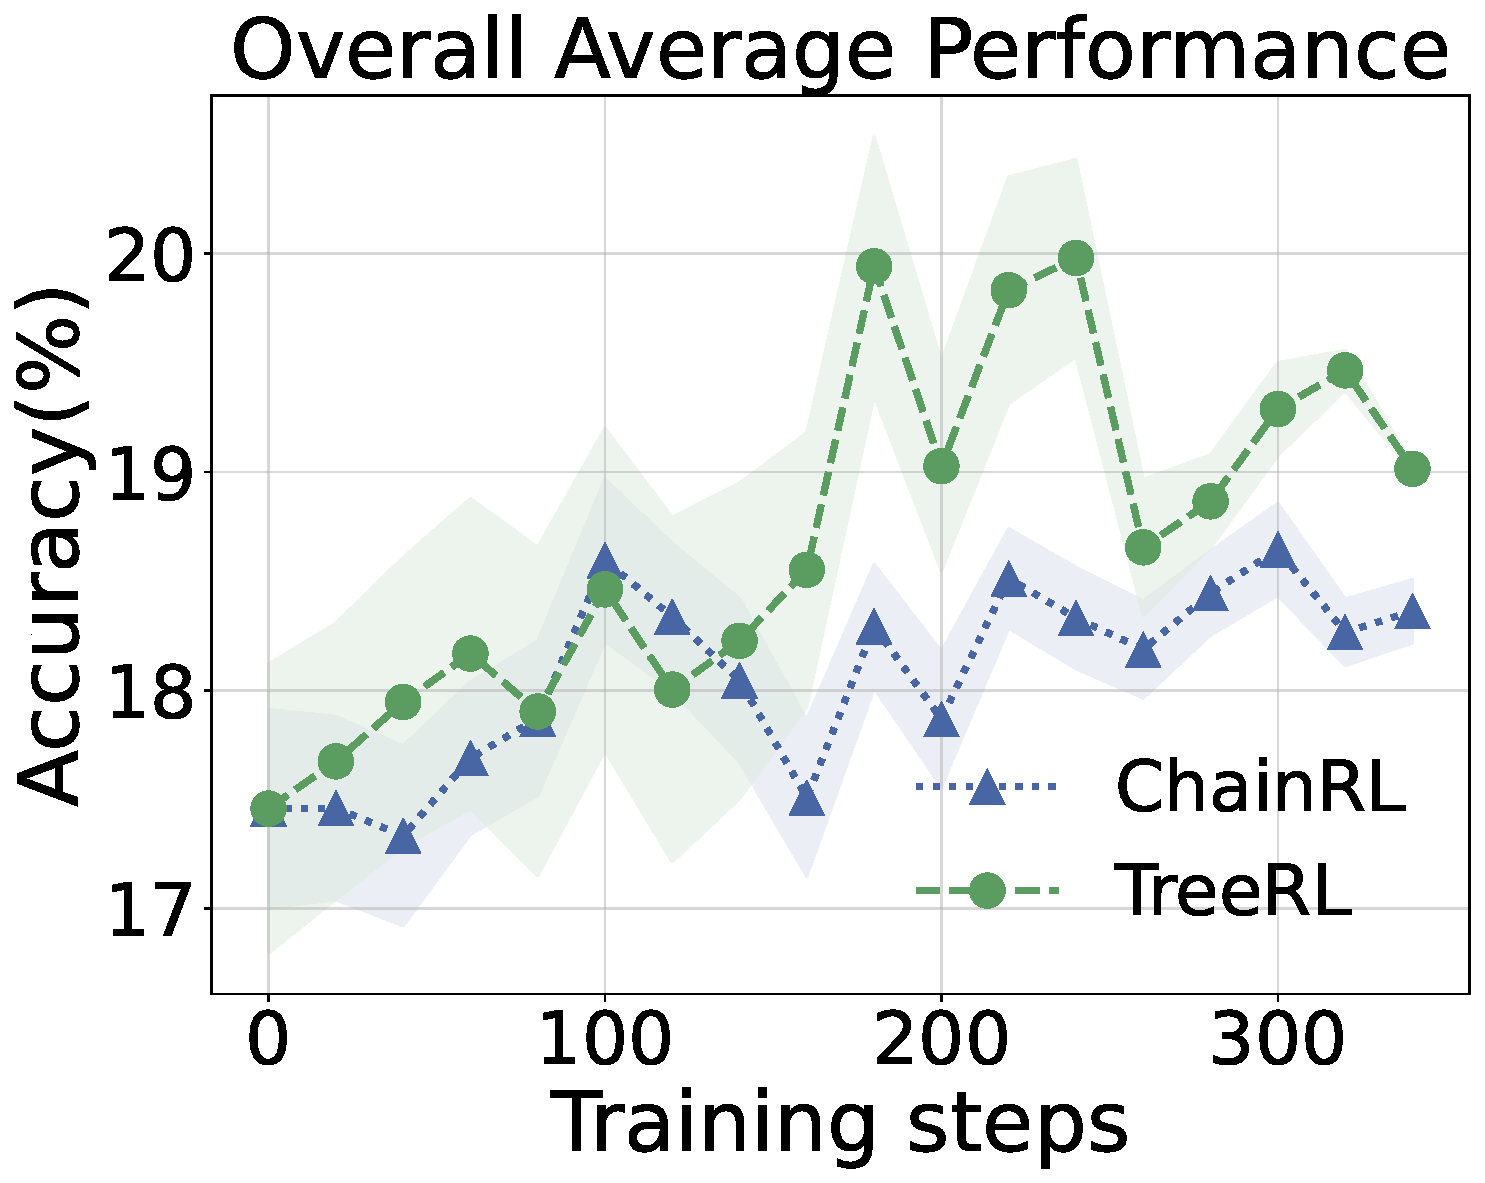
\includegraphics[width=\textwidth]{figure/glm-rlresult/average.pdf}
                \vspace{-5mm}
                \label{fig:fourth_image}
            \end{minipage}
            \hfill
            \begin{minipage}{0.32\textwidth}
                \centering
                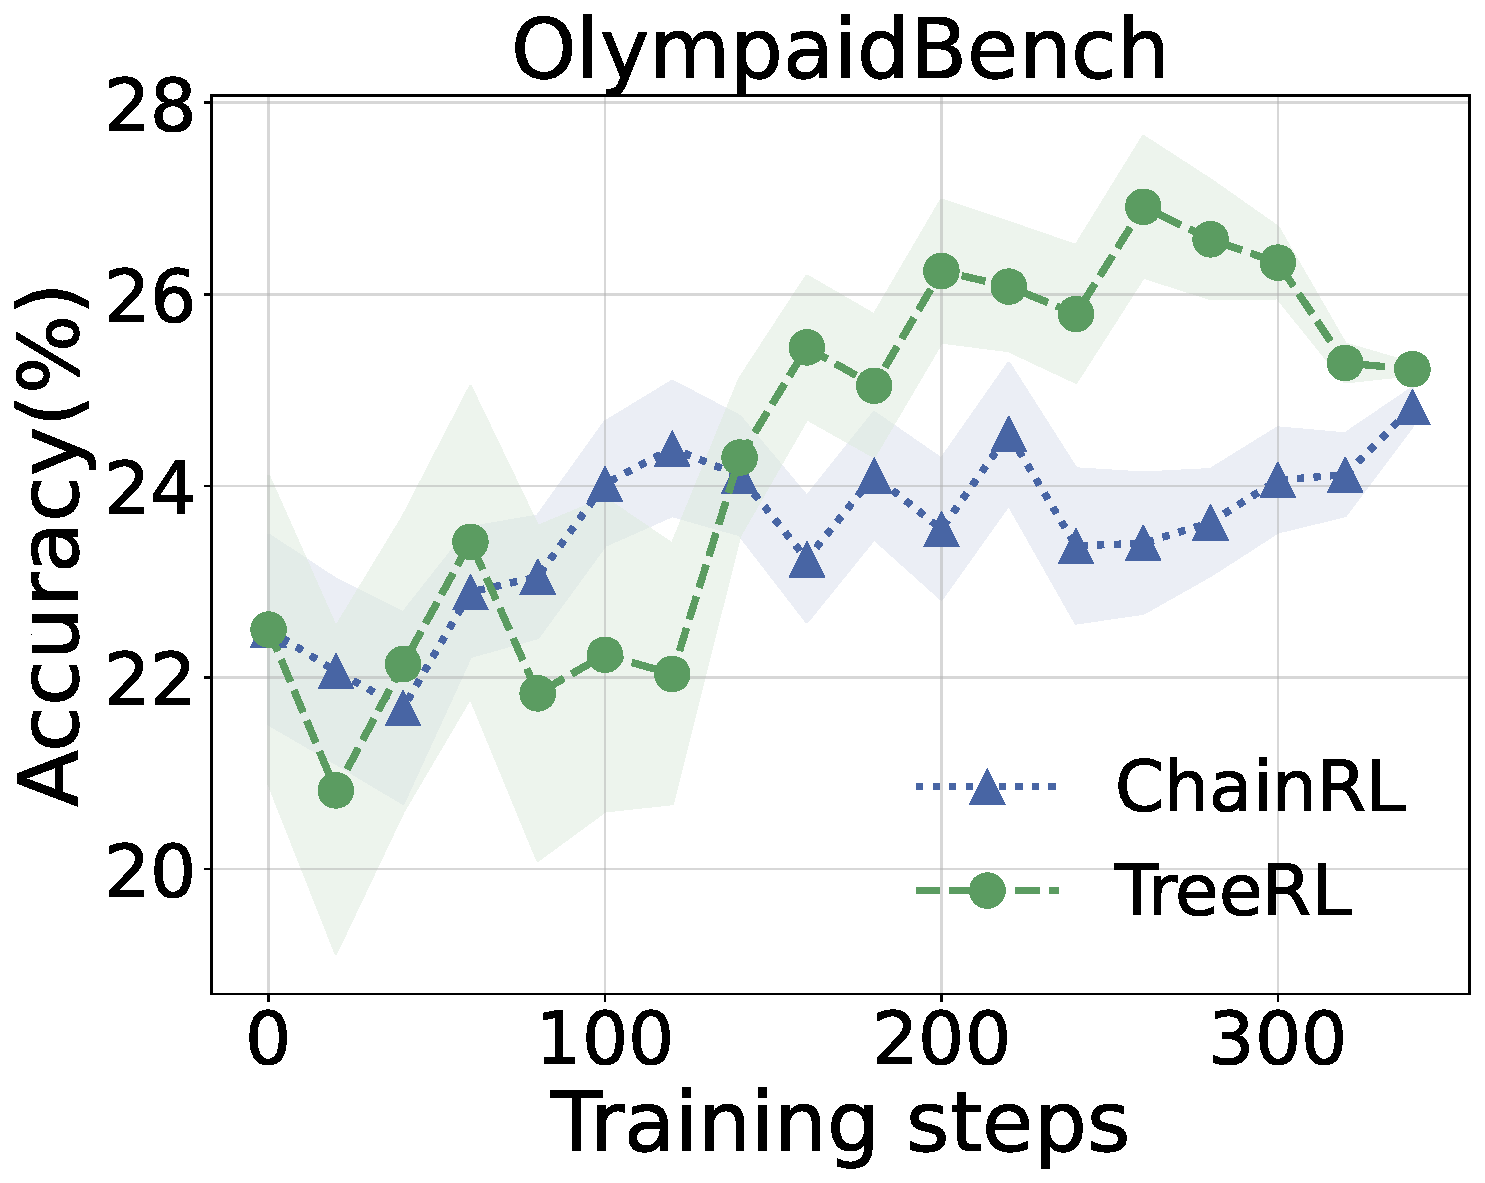
\includegraphics[width=\textwidth]{figure/glm-rlresult/olympaidbench.pdf}
                \vspace{-5mm}
                \label{fig:fifth_image}
            \end{minipage}
            \hfill
            \begin{minipage}{0.32\textwidth}
                \centering
                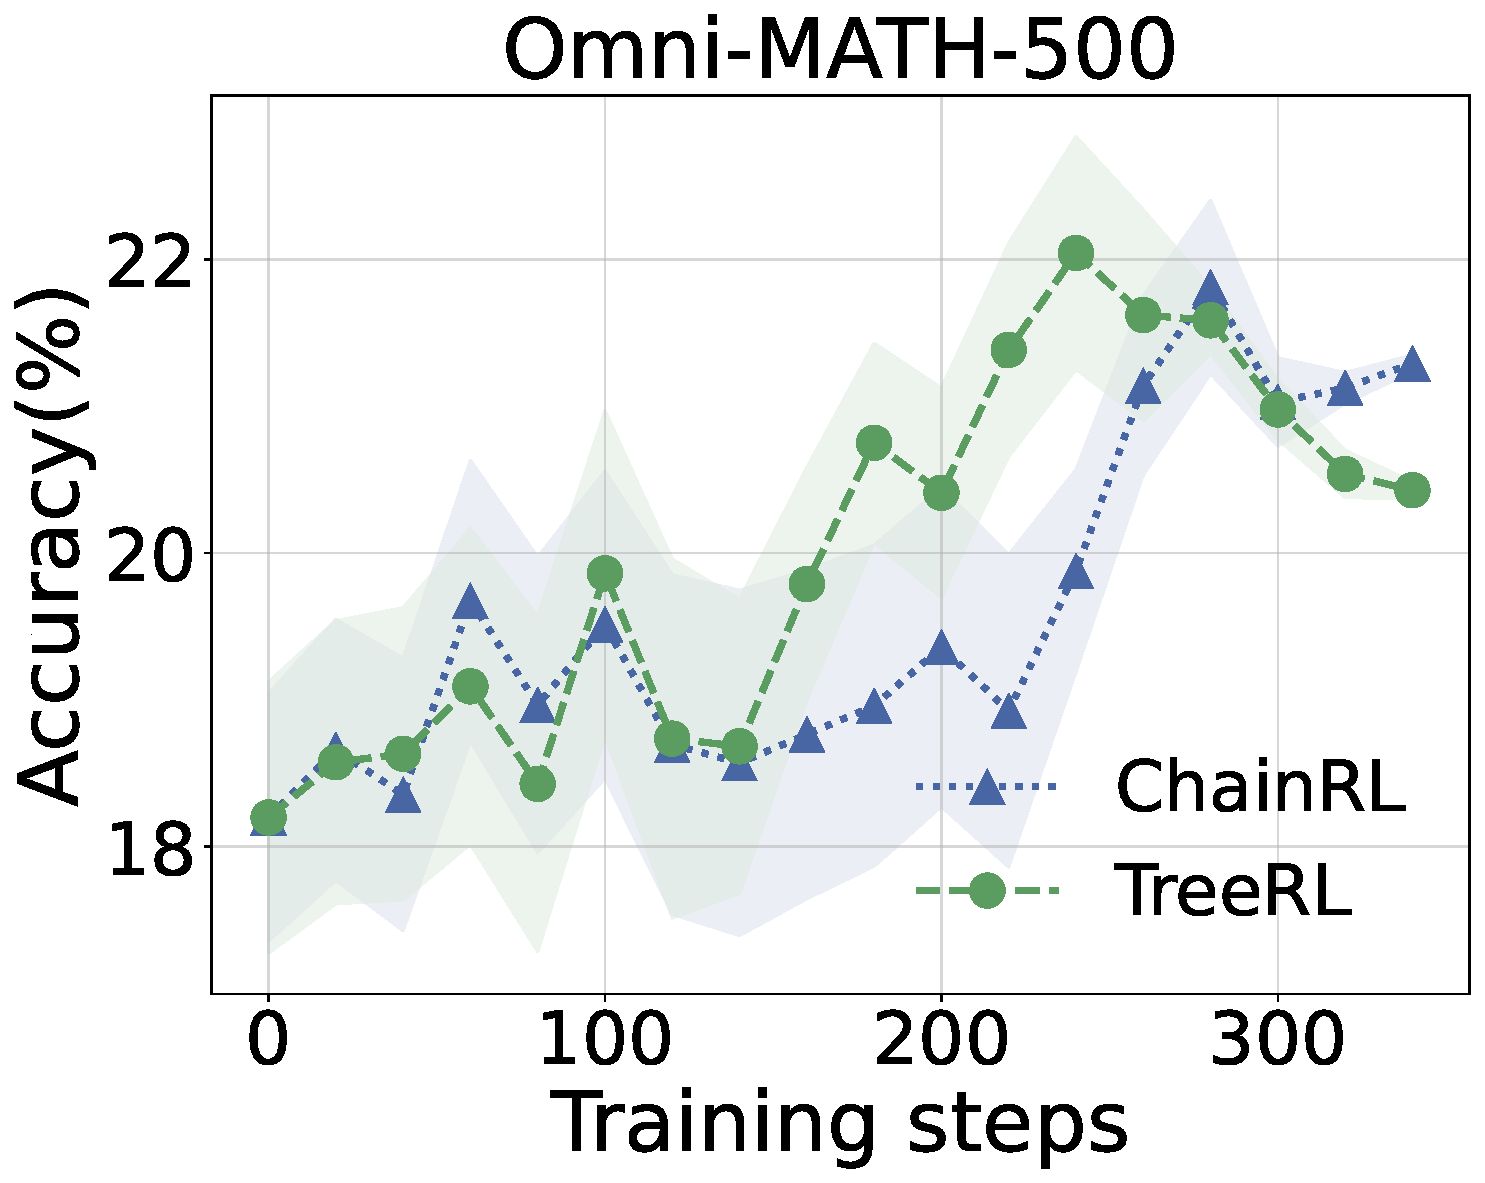
\includegraphics[width=\textwidth]{figure/glm-rlresult/omni.pdf}
                \vspace{-5mm}
                \label{fig:sixth_image}
            \end{minipage}
        \end{minipage}
    }
    \caption{Performance comparison between \model and ChainRL during training. We report the average performance across all six datasets (Left), OlympiadBench (Middle), and Omni-MATH-500 (Right). The results for the other benchmarks can be found in the \Cref{sec:appendix:other_benchmark}.}
    \label{fig: RL-results}
\end{figure*}


\subsection{Setup}
\label{sec:exp_setup}
\para{Training Details.} 
We train SFT models based on Qwen-2.5-14B~\citep{qwen2_5} and GLM4-9B~\citep{glm2024chatglm} as initialization for RL training and finetune them using the public dataset from \citep{hou2025advancing} for 2 epochs. 
For DeepSeek-R1-distilled-Qwen-2.5-7B, we directly use the open-source model from~\cite{guo2025deepseek} without further finetuning.
Then, to identify the best tree search setting for RL under a given inference cost, we investigate various combinations of hyperparameters $(M, N, L, T)$ using the trained Qwen-2.5-14B-SFT model on the Omni-MATH-500 dataset with PassRate as the target metric, and the results can be found in Table~\ref{tab:tree-parameter-evaluation} in the Appendix. 
% We set the baseline configuration with $N = L = T = 0$, which corresponds to the standard i.i.d. multi-chain sampling.
The baseline i.i.d multi-chain samplings correspond to setting $N = L = T = 0$.
% A hyperparameter search is conducted to identify the optimal configuration while ensuring that the inference costs remain comparable to those of multi-chain methods.

For the RL training, we compare the performance of RL using multi-chain sampling, referred to as ChainRL, to the proposed \model under the same inference cost derived from the previous search to ensure a fair comparison. 
For \model, we used sampling parameters $(M, N, L, T) = (6, 2, 1, 2)$, generating 30 responses per prompt. This is comparable to multi-chain sampling with 16 responses per prompt, given similar generation token budgets.  Each iteration used 16 prompts for a single gradient update, resulting in a batch size of 256 for ChainRL and 480 for \model. Therefore, \model actually performs reinforcement learning with the same inference cost but with more training computation during training. 
We use rule-based reward based on the correctness of the final answer, i.e., $+1$ for correct and $0$ for wrong.
The KL efficiency is set to $\beta = 10^{-4}$, with a learning rate of $1.5 \times 10^{-6}$. During sampling, the temperature is 1.2, the top-$p$ value is 0.95, and the maximum sequence length is 8,192.
For RL training, the training data all come from publicly available datasets, including MATH-train~\citep{hendrycksmath2021} and NuminaMath~\citep{li2024numinamath}, and we sample a subset for training.

\para{Evaluation}
% We evaluate our approach using two key metrics: PassRate for tree search and Pass@1 for RL training.
We use PassRate to evaluate the effectiveness of the proposed tree search algorithm. PassRate measures the potential of a model to reach at least one correct answer among all the generated solutions. 
It should be noted that we compare tree sampling and chain sampling under similar inference budgets, i.e., generation tokens.
% , but tree sampling generally leads to a than multi-chain sampling. 
Specifically, given an evaluation dataset $\mathcal{D}$, for each sample $d \in \mathcal{D}$, let $\mathcal{L}_d$ be the set of generated responses and $c(l)\in \{0,1\}$ be a binary indicator of correctness for a response $l$. The PassRate is computed as:
\[
\text{PassRate} = \frac{1}{|\mathcal{D}|} \sum_{d \in \mathcal{D}} \max_{l \in \mathcal{L}_d} c(l)
\]
For reinforcement learning, we evaluate the policy model on 6 challenging reasoning benchmarks using greedy sampling, 
% including MATH-500~\citep{}, Omni-MATH-500~\cite{}, AIME2024~\citep{}, AMC~\cite{}, and OlympiadBench~\citep{}. We report Accuracy(\%) for all benchmarks.
% We assess the performance on $5$ challenging competition-level mathematical reasoning datasets, 
including MATH\citep{hendrycksmath2021}, Omni-MATH \citep{gao2024omni}, AIME2024\citep{li2024numinamath}, AMC\citep{li2024numinamath}, OlympiadBench\citep{he2024olympiadbench}, and LiveCodeBench~\citep{jain2024livecodebench}. For the MATH dataset, we use a subset known as MATH500 based on the split defined by \citep{lightmanlet}. For Omni-MATH, we randomly sample a subset for evaluation, named Omni-MATH-500, which consists of 500 examples for efficient yet comprehensive assessment. Each dataset undergoes multiple evaluations to minimize variance; for instance, we evaluate MATH500 and Omni-MATH-500 three times each, while AIME is evaluated 32 times, considering AIME2024 consists of only 30 questions. For LiveCodeBench, we report the performance using the data between 202407 to 202411.


% \subsection{Main Results}


\subsection{Results of \treemodel}
\Cref{tab:tree-parameter-evaluation} shows the overall performance on Omni-MATH-500 and illustrates the efficiency and effectiveness trade-off across different sampling methods. 
\treemodel demonstrates a significant advantage over the baseline multi-chain sampling method and the MCTS method under the same inference cost. And \treemodel shows consistently better performance across different generation costs and outperforms the multi-chain sampling by around 3\% in PassRate. Compared to MCTS, \treemodel demonstrates a more significant advantage, with the margin widening as the inference cost increases.

\subsection{Results on RL training}
Table~\ref{tab:experiments} presents the performance of various sampling strategies in RL training. Notably, \model equipped with \treemodel sampling outperforms traditional multi-chain sampling across different benchmarks. In particular, Figure~\ref{fig: RL-results} illustrates the evaluation performance over various training steps. While both sampling strategies exhibit similar performance during the early stages of training, \model begins to show an advantage around 100 steps and continues to improve consistently. This indicates that the \model achieves better prompt efficiency by delivering enhanced performance with the same number of training prompts. Overall, these results underscore the promise of integrating tree search and process supervision into RL training. 
It is observed that both RL methods show only minor improvements over the SFT baseline. This could be due to the fact that we selected the RL training data based on Qwen-2.5-14B, which is likely much easier for the R1-Distilled-Qwen-2.5-7B model, thereby limiting the potential performance gains in RL. 


% \subsubsection{Tree search}
% \label{sec:tree_search}

% \para{Performance} We conduct comprehensive experiments on Omni-MATH-500 dataset to evaluate different parameter combinations $(m,n,l,t)$. We choose this dataset as it poses more challenging problems compared to MATH-500, where most settings achieve near-perfect pass@k rates for $k\geq16$ (see \Cref{sec:appendix:entropy_math}).
% The overall performance is illustrated in Figure~\ref{fig:entropy-tree-algorithm}. 
% Similarly, improvements in problem-solving performance on the Omni-MATH-500 dataset are depicted in \Cref{fig:tree_vs_mcts_iid}. This graph summarizes the advantage of using entropy-tree search over i.i.d sampling in yielding higher pass rates at equivalent computational costs.


% The efficiency of the entropy-tree search in terms of leaf sampling is demonstrated in \Cref{fig:tree_vs_iid_leaf_num}, which shows that our method can produce approximately \textbf{double} the number of leaf nodes for the same token cost when compared to the baseline independent and identically distributed (i.i.d.) sampling method.


% The overall performance is illustrated in \Cref{fig:tree_vs_mcts_iid}.
% Notably, in all the settings tested, the repetition rate of solutions remained low, ranging from 0.1\% to 0.2\%, highlighting the method's capability in generating diverse solutions without redundant iterations. \Cref{tab:parameter-evaluation} provides a summary of the effects of these parameters on solution diversity (measured by leaf number) and effectiveness (measured by pass rate).

% \begin{table}[ht]
%     \centering
%     \caption{Overview of $(M,N,L,T)$ Parameter Evaluation and Their Impact on Leaf Num and Performance on Omni-MATH-500. The table reports the leaf number, pass rate, and total generated tokens under different parameter combinations for $k=16$ and $k=64$.}
%     \label{tab:tree-parameter-evaluation}
%     \resizebox{0.45\textwidth}{!}{%
%         \begin{tabular}{@{}cccccc@{}}
%             \toprule[1.2pt]
%             \multicolumn{1}{c}{$\textbf{(M, N, L, T)}$} & \textbf{\#Leaf} $\uparrow$ & \textbf{Pass@$K$} $\uparrow$ & \textbf{\#Token} $\downarrow$ \\
%             \midrule
%             \multicolumn{4}{c}{\textit{$k=16$}} \\
%             \midrule
%             multi-16      & 16 & 52.4 & 19858 \\
%             (8, 3, 1, 1)  & 32 & 58.4 & 25223 \\
%             (7, 2, 1, 2)  & 35 & 59.2 & 26200 \\
%             (6, 2, 2, 1)  & 30 & 54.4 & 20537 \\
%             (6, 2, 1, 2)  & 30 & 56.9 & 22268 \\
%             (5, 3, 1, 2)  & 35 & 58.6 & 25269 \\
%             (5, 2, 1, 3)  & 35 & 56.0 & 25210 \\
%             (5, 3, 2, 1)  & 35 & 58.0 & 22668 \\
%             (5, 1, 2, 3)  & 35 & \textbf{58.6} & 21895 \\
%             \midrule
%             \multicolumn{4}{c}{\textit{$k=64$}} \\
%             \midrule
%             multi-64      & 64 & 67.4 & 79367 \\
%             (16, 2, 2, 2) & 144 & 70.0 & 88257 \\
%             (16, 4, 1, 2) & 144 & 71.4 & 101744 \\\
%             (16, 2, 1, 4) & 144 & 72.6 & 100468 \\
%             (9, 5, 1, 3)  & 144 & 71.9 & 98193 \\
%             (9, 3, 1, 5)  & 144 & 71.6 & 97193 \\
%             (8, 8, 1, 2)  & 136 & 70.7 & 92946 \\
%             (8, 4, 1, 4)  & 136 & 69.7 & 90015 \\
%             (8, 8, 2, 1)  & 136 & 68.6 & 79582 \\
%             (8, 4, 2, 2)  & 136 & \textbf{71.0} & 77768 \\
%             (8, 2, 2, 4)  & 136 & 69.4 & 76750 \\
%             \bottomrule[1.2pt]
%         \end{tabular}
%     }
% \end{table}


\subsection{Ablation Study on \treemodel Sampling}
\vpara{Effects of entropy-based forking.} Table~\ref{tab:entropy-fork-token-ablation} illustrates the performance across different strategies when forking new branches in tree expansion. 
% Compared to randomly selecting tokens for expansion, forking from tokens with high entropy 
\treemodel shows better PassRate than random forking with fewer generation tokens, which demonstrates the advantage of \treemodel. In addition, both tree sampling strategies outperform multi-chain sampling, offering the potential of tree search.
% In Section~\ref{}, \treemodel forks new branches from tokens with high entropy. Table~\ref{tab:entropy-fork-token-ablation} illustrates 

\begin{table}[t]
    \centering
    \caption{Ablation of \treemodel on Omni-MATH-500. We compare forking branches using random and entropy-based strategies on Qwen-2.5-14B-SFT. $(16,0,0,0)$ corresponds to multi-chain sampling. \textit{Entropy} denotes whether to use entropy-based forking strategy. \treemodel model shows better PassRate performance yet with fewer generation tokens.}
    \resizebox{0.5\textwidth}{!}{
        \begin{tabular}{cccc}
        \toprule[1.2pt]
        $(M,N,L,T)$ & Entropy & PassRate $\uparrow$ & \#Token $\downarrow$ \\
        \midrule
        % \multirow{2}{*}{$(6,2,1,2)$} 
        $(6,2,1,2)$ & $\checkmark$ & \textbf{56.9} & \textbf{22268} \\
        $(6,2,1,2)$ & \ding{55} & 54.8 & 24213 \\
        $(16,0,0,0)$ & - & 52.4 & 19858 \\
        \midrule
        % \multirow{2}{*}{$(8,4,2,2)$}
        $(8,4,2,2)$ & $\checkmark$ & \textbf{71.0} & \textbf{77768} \\
        $(8,4,2,2)$ & \ding{55} & 70.0 & 89452 \\
        $(64,0,0,0)$ & - & 67.4 & 79367 \\
        \bottomrule[1.2pt]
        \end{tabular}
    }
    \label{tab:entropy-fork-token-ablation}
\end{table}



\vpara{Case study on forking tokens.} 
To help better understand \treemodel, we conduct case studies to analyze what type of tokens tend to be selected.
% Our analysis of forking points focuses on two key aspects: frequency and position.
We examine frequency by identifying the top-10 tokens that most often serve as forking points, and the results are illustrated in \Cref{fig:top_10_tokens}. It can be observed that mathematical operators ($\backslash($), logical conjunctions, and transitional terms (``Since'', ``But'') are frequently selected. Notably, the token ``wait'' appears frequently, as o1-like models often use it for self-reflection steps. 
% Second, we study the position of these forked tokens in their branches. 
% In \Cref{fig:forked_token_position_ratio_histogram}, we plot the relative positions of forking points, calculated as the ratio between a token's forking position and its branch length. 
% The resulting distribution shows a roughly uniform pattern, which supports our assumptions presented in \Cref{sec:appendix:proof}.

\begin{figure}[t]
    \centering
    %\includegraphics[width=0.95\linewidth]{figure/top_10_tokens_by_proportion_omni_math_500_entropy_guided.pdf}
    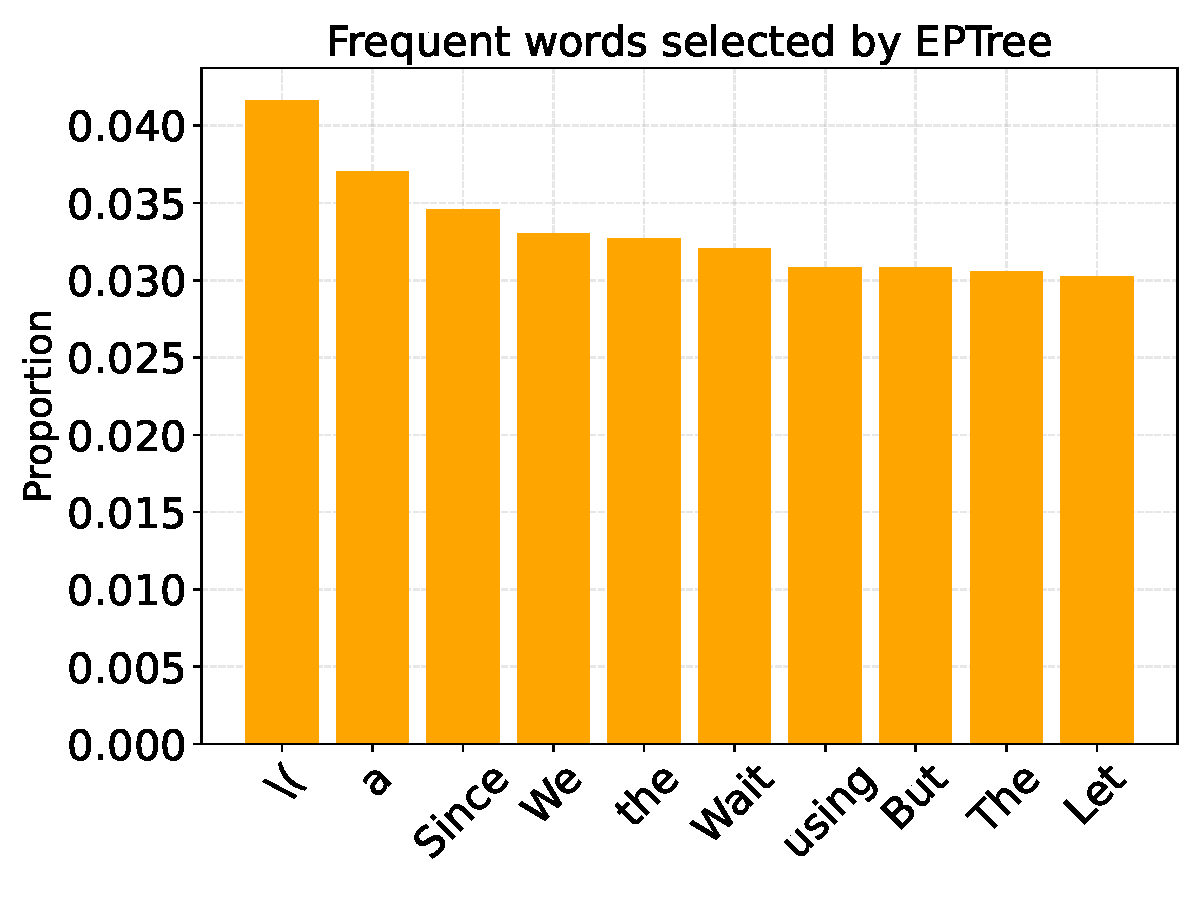
\includegraphics[width=0.95\linewidth]{figure/word_frequency_figure.pdf}
    \caption{Frequent words of sampled forking tokens in \treemodel sampling on Omni-MATH-500.}
    \label{fig:top_10_tokens}
\end{figure}


\hide{
\begin{table*}[ht]
    \caption{Ablation on the effectiveness of different process signals for RL training using Qwen2.5-14B. $G_A$ and $L_A$ denote the global and local advantages, respectively. $n$ refers to the number of leaf nodes that can be reached from the given step. \#Response denotes the number of responses used for training.}
    \centering
    \resizebox{\textwidth}{!}{%
    \begin{tabular}{cc|cccccc|c}
    \toprule[1.2pt]
       Reward  & \#Responses & MATH500 & \makecell{Omni-MA\\TH-500} & AIME2024 & AMC & \makecell{Olympiad\\Bench} & LiveCodeBench & Avg \\
    \midrule
    $(G_A + L_A)/\sqrt{n}$ & 30  & \textbf{81.7} & \textbf{36.7} & \textbf{28.0} & \textbf{55.9} &  \textbf{44.6} & \textbf{20.8} &\textbf{44.5} \\
    $G_A+L_A$ & 30 & 81.5 & 32.0 & 24.1 & 56.2 & 42.1 & & \\
    $G_A$ & 30 &  80.1 & 35.1 & 24.7 & 55.5 & 42.8 & 20.7 & 43.2 \\
    $(G_A + L_A)/\sqrt{n}$ & 16 & 80.1 & 32.5 & 24.5 & 52.9 & 41.7 & 15.8 & 41.3 \\
    % \rowcolor{airforceblue}
     \bottomrule[1.2pt]
    \end{tabular}%
    }
    \label{tab:ablation_rl}
\end{table*}
}

\begin{table*}[ht]
    \caption{Ablation on the effectiveness of different process signals for RL training using Qwen2.5-14B. $G_A$ and $L_A$ denote the global and local advantages, respectively. $n$ refers to the number of leaf nodes that can be reached from the given step. \textit{\#Response} denotes the number of responses used for training.}
    \centering
    \resizebox{\textwidth}{!}{%
    \begin{tabular}{cc|cccccc|c}
    \toprule[1.2pt]
       Reward  & \#Responses & MATH500 & \makecell{Omni-MA\\TH-500} & AIME2024 & AMC & \makecell{Olympiad\\Bench} & \makecell{LiveCode\\Bench} & Avg Gain \\
    \midrule
    $(G_A + L_A)/\sqrt{n}$ & 30  & \textbf{81.7} & \textbf{36.7} & \textbf{28.0} & 55.9 & \textbf{44.6} & \textbf{20.8} & - \\
    $G_A+L_A$ & 30 & 81.5 & 32.0 & 24.1 & \textbf{56.2} & 42.1 & 19.7 & -1.9 $\downarrow$ \\
    %$G_A$ & 30 &  80.1 & 35.1 & 24.7 & 55.5 & 42.8 & 20.7 & -1.3 $\downarrow$ \\
    $G_A / \sqrt{n}$ & 30 &  80.1 & 35.1 & 24.7 & 55.5 & 42.8 & 20.7 & -1.3 $\downarrow$ \\
    $(G_A + L_A)/\sqrt{n}$ & 16 & 80.1 & 32.5 & 24.5 & 52.9 & 41.7 & 15.8 & -3.2 $\downarrow$ \\
     \bottomrule[1.2pt]
    \end{tabular}%
    }
    \label{tab:ablation_rl}
\end{table*}

% \begin{proof}
%     see \Cref{sec:appendix:proof}.
% \end{proof}

\subsection{Ablation on \model}
To test the effectiveness of process supervision in \model, we compare different designs of process supervision signals. Additionally, since the \model uses more traces than RL with multi-chain sampling, we also evaluate how the increased training cost impacts performance. The results are presented in Table~\ref{tab:ablation_rl}.
The results demonstrate that RL with reweighted local and global advantage achieves the best performance. Removing either component could lead to a decline in performance. Moreover, using a subset of sampled responses shows less improvement compared to utilizing the entire set. This suggests that, in addition to higher PassRate and process supervision, tree search enhances RL performance by enabling more training within the same inference cost.


% 16 * n => 32 * n
% tree process => tree chain
% 6, 2, 1, 2 use all => use partial
